\documentclass[]{article}
\usepackage[a4paper,margin=0.5cm,landscape]{geometry}
\usepackage{amsmath}
\usepackage{amsfonts}
\usepackage{amssymb}
\usepackage{mathtools}
\usepackage{amsthm}
\usepackage[many]{tcolorbox}
\usepackage{listings}
\usepackage{multicol}
\usepackage{graphicx}

\usepackage{xpatch}
\makeatletter
\xpatchcmd{\@thm}{\thm@headpunct{.}}{\thm@headpunct{}}{}{}
\makeatother

\newtheorem*{green}{}
\newtheorem*{red}{}
\newtheorem*{blue}{}
\newtheorem*{yellow}{}

\tcolorboxenvironment{green}{
	colback=green!5!white,
	boxrule=0pt,
	boxsep=1pt,
	left=2pt,right=2pt,top=2pt,bottom=2pt,
	oversize=2pt,
	sharp corners,
	before skip=\topsep,
	after skip=\topsep,
}

\tcolorboxenvironment{red}{
	colback=red!5!white,
	boxrule=0pt,
	boxsep=1pt,
	left=2pt,right=2pt,top=2pt,bottom=2pt,
	oversize=2pt,
	sharp corners,
	before skip=\topsep,
	after skip=\topsep,
}

\tcolorboxenvironment{blue}{
	colback=blue!5!white,
	boxrule=0pt,
	boxsep=1pt,
	left=2pt,right=2pt,top=2pt,bottom=2pt,
	oversize=2pt,
	sharp corners,
	before skip=\topsep,
	after skip=\topsep,
}

\tcolorboxenvironment{yellow}{
	colback=yellow!5!white,
	boxrule=0pt,
	boxsep=1pt,
	left=2pt,right=2pt,top=2pt,bottom=2pt,
	oversize=2pt,
	sharp corners,
	before skip=\topsep,
	after skip=\topsep,
}

\begin{document}	
	
\begin{multicols}{3}
\begin{minipage}[t]{.31\textwidth}

\begin{green}
\begin{tabular}{c|c}
	proposition & Stat. that can either be true or false\\
	\hline
	(ground) formula & $p_1 \lor p_2 \land (p_3 \rightarrow p_4)$ \\
	\hline
	literal & $p_1$; $\lnot p_2$ \\
	\hline
	clause & $p_1 \lor \lnot p_2$ \\
	\hline
	horn clause & at most 1 pos. literal \\
	\hline
	term & $f(x,a)$ \\
	\hline
	atomic formula & $p(f(x,a), g(y))$ \\
	\hline
	formula & $\forall x \exists y (p(f(x,a), g(y)))$ \\
	\hline
	signature & sorts, constants,\\
	& functions, predicate symbols \\
	\hline
	CNF & $\bigwedge_i \bigvee_j L_{i,j}$\\
\end{tabular}
\end{green}

\subsubsection*{Precedence}
in this order from left to right: $\top, \bot, \lnot, \land, \lor, \rightarrow, \leftrightarrow$

\subsubsection*{Polarity}
\begin{blue}
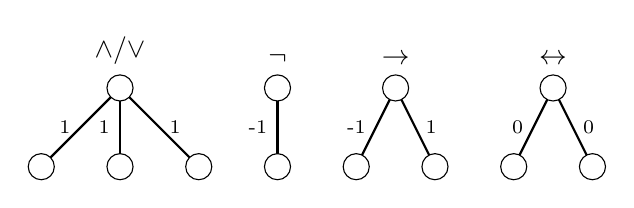
\begin{tikzpicture}
	\tikzstyle{node} = [circle, draw=black, fill=white];
	
	\draw[thick] (1,1) -- (0,0) node[draw=none,fill=none,font=\scriptsize,midway,left] {1};
	\draw[thick] (1,1) -- (1,0) node[draw=none,fill=none,font=\scriptsize,midway,left] {1};
	\draw[thick] (1,1) -- (2,0) node[draw=none,fill=none,font=\scriptsize,midway,right] {1};
	
	\draw[thick] (3,1) -- (3,0) node[draw=none,fill=none,font=\scriptsize,midway,left] {-1};;
	
	\draw[thick] (4.5,1) -- (4,0) node[draw=none,fill=none,font=\scriptsize,midway,left] {-1};
	\draw[thick] (4.5,1) -- (5,0) node[draw=none,fill=none,font=\scriptsize,midway,right] {1};

	\draw[thick] (6.5,1) -- (6,0) node[draw=none,fill=none,font=\scriptsize,midway,left] {0};
	\draw[thick] (6.5,1) -- (7,0) node[draw=none,fill=none,font=\scriptsize,midway,right] {0};
	
	\node[node, label=$\land$/$\lor$] at (1, 1) (aotop) {};
		\node[node] at (0, 0) (aol) {};
		\node[node] at (1, 0) (aom) {};
		\node[node] at (2, 0) (aor) {};
		
	\node[node, label=$\lnot$] at (3, 1) (ntop) {};
		\node[node] at (3, 0) (nm) {};
	
	\node[node, label=$\rightarrow$] at (4.5, 1) (itop) {};
		\node[node] at (4, 0) (il) {};
		\node[node] at (5, 0) (ir) {};
		
	\node[node, label=$\leftrightarrow$] at (6.5, 1) (etop) {};
		\node[node] at (6, 0) (el) {};
		\node[node] at (7, 0) (er) {};

\end{tikzpicture}

$p$ ... pos. pure $\implies p \mapsto 1$; $p$ ... neg. pure $\implies p \mapsto 0$

\end{blue}

\subsubsection*{Naming}
\begin{blue}
Replace subformula $s$ with name $n$ and add $n\leftrightarrow s$ (if $s$ occurs only positively $n\rightarrow s$ elif $s$ occurs only negatively $s \rightarrow n$).
\end{blue}

\subsubsection*{Unit Propagation}
\begin{blue}
Clauses of the form $p$ are solved by setting $p \mapsto 1$ and propagating. Same with $\lnot p$ where $p \mapsto 0$.
\end{blue}

SAT is NP-complete.

\subsubsection*{GSAT}
\begin{red}
\begin{verbatim}
repeat max_tries times:
    I = random interpretation
    if I models S return I
    repeat max_flip times:
        p = variable s.t. flip(I,p)
            satisfies max clauses in S
        I = flip(I, p)
        if I models S return I
return don't know	
\end{verbatim}
\end{red}

\end{minipage}\hfil

\begin{minipage}[t]{.31\textwidth}
\subsubsection*{WSAT}
\begin{red}
\begin{verbatim}
repeat max_tries times:
    I = random interpretation
    if I models S return I
    repeat max_flip times:
        randomly select clause C in S
                   s.t. I does not model C
        randomly select variable p in C
        I = flip(I, p)
        if I models S return I
return don't know	
\end{verbatim}
\end{red}

\begin{green}
Two interpretations are \textbf{$\mathbf{\bar{x}}$-variants} if they coincide on all symbols and all variables not occurring in $\bar{x}$.
\end{green}

\begin{green}
$\mathbf{(\forall x A)^I = 1}$ iff for all $\bar{x}$-variants $I'$ of $I$ we have $(A)^{I'} = 1$.

$\mathbf{(\exists x A)^I = 1}$ iff for some $\bar{x}$-variants $I'$ of $I$ we have $(A)^{I'} = 1$.
\end{green}

\begin{green}
$A$ with free variables $\bar{x}$ is \textbf{sat in an interpretation} $I$ if for some $\bar{x}$-variants $I'$ we have $I'\models A$.

$A$ with free variables $\bar{x}$ is \textbf{valid in an interpretation} $I$ if for every $\bar{x}$-variants $I'$ we have $I'\models A$.

$A$ is \textbf{valid} iff it is valid in every interpretation ($\iff \lnot A$ is unsat.)
\end{green}

\subsubsection*{Congruence Closure}
\begin{blue}
	For every equation $s=t$ union $[s]$ and $[t]$ and function propagate. If $s \not= t$, but $[s] = [t]$ report unsat, else report sat.
\end{blue}

\subsubsection*{DPLL}
\begin{red}
\begin{verbatim}
abstract by renaming literals
use SAT solver to find model
if no model found return unsat
else solve resulting unit clause problem
if solution exists return sat
else rule out this model and go back to SAT solver
\end{verbatim}
\end{red}

\subsubsection*{Theory of Arrays}
\begin{blue}
read without write: $read(A,x) \rightsquigarrow f_A(x)$

read with write: $read(write(A,x,v),y) \rightsquigarrow x=y \land F[v]$

or \hspace{4cm} $\rightsquigarrow x\not= y \land F[read(A,y)]$
\end{blue}

\end{minipage}\hfil

\begin{minipage}[t]{.31\textwidth}

\subsubsection*{Combining Theories}
\begin{blue}
Rename subterms s.t. each formula is only in one theory.
\end{blue}

\subsubsection*{Decision Procedure for Combined Theories}
\begin{blue}
Discover shared $u=v$ (or $\bigvee_k u_k = v_k$ then use splitting) and pass to other theories.
\end{blue}

\begin{green}
Theory $\mathcal{T}$ with signature $\Sigma$ is \textbf{stably infinite} if $\forall F \in \mathcal{T}$ ... sat $\exists I$ ... $\mathcal{T}$-interpretation: $I \models F$ and $I$ has domain of infinite cardinality.

Theory $\mathcal{T}$ is \textbf{convex} if $\forall F \in \mathcal{T}$ .. conjunction of $\mathcal{T}$-literals ($F \rightarrow \bigvee_{j=1}^k(u_j = v_j) \implies \exists j\in\{1,...,k\}: F \rightarrow u_j = v_j$).

\textbf{Soundness:} conclusion is logical consequence of premises

\textbf{Completeness:} every unsat $S$ has derivation of $\square$ in $\mathbb{I}$

\textbf{Well-founded:} $\not\exists$ infinite decreasing chain of atoms

\textbf{Well-behaved:} select either neg. literal or all max. literals

\textbf{Fair:} $\forall$ $\frac{F_1...F_n}{F}$ ... inference with $F_1,...,F_n \in S_\omega \exists i: F \in S_i$
\end{green}

$\mathcal{T}_E$, $\mathcal{T}_Q$ are convex. $\mathcal{T}_Z$, $\mathcal{T}_A$ are not convex.

\subsubsection*{TPTP Syntax}
\begin{green}
	
\begin{verbatim}
fof(name, axiom/conjecture/hypothesis, formula).
\end{verbatim}

\begin{tabular}{c|c}
	$\top, \bot$ & \verb|$true, $false|\\
	\hline
	$\lnot a$ & \verb|~a|\\
	\hline
	$a_1 \land ... \land a_n$ & \verb|a1&...&an|\\
	\hline
	$a_1 \lor ... \lor a_n$ & \verb@a1|...|an@\\
	\hline
	$a_1 \rightarrow a_2$ & \verb|a1=>a2|\\
	\hline
	$\forall x_1 ... \forall x_n (a)$ & \verb|![X1,...,Xn]:a|\\
	\hline
	$\exists x_1 ... \exists x_n (a)$ & \verb|?[X1,...,Xn]:a|\\
	\hline
\end{tabular}
\end{green}

\subsubsection*{Binary Resolution}
\begin{blue}
\begin{align*}
	\frac{\underline{p}\lor C_1 \hspace{.5cm} \underline{\lnot p} \lor C_2}{C_1 \lor C_2} (BR) \hspace{1cm} \frac{\underline{L}\lor \underline{L} \lor C}{L \lor C} (Fact)
\end{align*}
\end{blue}

\begin{green}
$\mathbf{>^{bag}}$ is the smallest transitive relation on bags of $X$ s.t.
\begin{align*}
	\{x,y_1,...,y_n\} >^{bag} \{x_1,...,x_m,y_1,...,y_n\}\\
	\text{ if } \forall i\in\{1,...,m\}: x>x_i
\end{align*}
\end{green}

\begin{green}
A clause $C \in S$ is called \textbf{redundant} in $S$ if it is a logical consequence of clauses in $S$ strictly smaller than $C$.
\end{green}

\end{minipage}

\newpage

\begin{minipage}[t]{.31\textwidth}
\begin{green}
	\textbf{Limit} $\mathbf{S_\omega} = \bigcup_{i\in\mathbb{N}} \bigcap_{j\geq i} S_j$ ... set of all persistent clauses
\end{green}

\begin{green}
$S$... set of clauses is \textbf{saturated up to redundancy} if $\forall \frac{C_1...C_n}{C} ... \mathbb{I}$-inference with premises in $S$, either $C \in S$ or $C$ is redundant w.r.t. $S$.
\end{green}

\begin{green}
$(s' = t') >_{lit} (s=t) \iff \{s',t'\}>_{bag}\{s,t\}$ and

$(s' \not= t') >_{lit} (s\not=t) \iff \{s',t'\}>_{bag}\{s,t\}$.
\end{green}

\subsubsection*{Superposition}
\begin{blue}
\begin{align*}
	\frac{\underline{l=r} \lor C \hspace{.5cm} \underline{s[l]=t} \lor D}{s[r]=t \lor C \lor D} (Sup-right)\\
	\frac{\underline{l=r} \lor C \hspace{.5cm} \underline{s[l]\not=t} \lor D}{s[r]\not=t \lor C \lor D} (Sup-left)\\
\end{align*}
where (i) $l>r$, (ii)$s[l]>t$, (iii) $l=r$ is strictly greater than any literal in $C$, (iv) (only for sup-right) $s[l]=t$ is greater than or equal to any literal in $D$
\begin{align*}
	\frac{\underline{s\not= s} \lor C}{C} (ER) && \frac{\underline{s=t} \lor s=t' \lor C}{s=t \lor t\not= t' \lor C} (EF)
\end{align*}
where (i) $s>t\geq t'$, (ii) $s=t$ is greater than or equal to any literal in $C$.
\end{blue}

\begin{green}
$>$ on terms is \textbf{simplification ordering} if well-founded; monotonic (if $l>r$ then $s[l]>s[r]$); stable under substitutions (if $l>r$ then $l\theta > r\theta$).
\end{green}


\subsubsection*{Knuth-Bendix Ordering (KBO)}
\begin{green}
given signature $\Sigma$, precedence relation $\gg$ and weight function $w:\Sigma \rightarrow \mathbb{N}$:

Ground term weight: $|g(t_1,...,t_n)| = w(g)+ \sum_{i=1}^{n}|t_i|$.

$g(t_1,...,t_n) >_{KBO} h(s_1,...,s_m)$ if
\begin{enumerate}
	\item $|g(t_1,...,t_n)| > |h(s_1,...,s_m)|$ or
	\item $|g(t_1,...,t_n)| = |h(s_1,...,s_m)|$ and
	\begin{enumerate}
		\item $g\gg h$ or
		\item $g=h$ and for some $1 \leq i \leq n$ we have $t_1=s_1,...,t_{i-1}=s_{i-1}$ and $t_i > s_i$.
	\end{enumerate}
\end{enumerate}
\end{green}

\end{minipage}\hfil

\begin{minipage}[t]{.31\textwidth}
	
\begin{green}
	\textbf{weight function} $w:\Sigma \cup Vars \rightarrow \mathbb{N}$ satisfies:
	\begin{itemize}
		\item $\forall x$ ... variables: $ w(x) = v_0 (> 0)$
		\item $\forall a$ ... constant: $w(a) \geq v_0 $
		\item $\exists f$ ... unary function$: w(f)=0$ then $\forall g\not=f$ ... function: $f \gg g$.
	\end{itemize}
\end{green}
	
\subsubsection*{Demodulation}
\begin{align*}
	\frac{\underline{l=r} \hspace{0.2cm} \underline{s[l]=t} \lor D}{s[r]=t \lor D}(Sup)
\end{align*}
then the right premise becomes redundant.

\begin{green}
\textbf{substitution} $\mathbf{\theta}$ is a mapping from variables to terms such that the set $\{x | \theta(x) \not= x\}$ is finite and is denoted by $\{x_1 \mapsto t_1, ..., x_n \mapsto t_n\}$.

\textbf{unifier} of $s_1$ and $s_2$ is substitution $\theta$ s.t. $s_1\theta = s_2\theta$.

Unifier $\theta$ of $s_1$ and $s_2$ is a \textbf{mgu} if $\forall\theta' \exists\tau$ such that $\theta\tau = \theta'$.
\end{green}

\subsubsection*{Find mgu}
\begin{red}
\begin{verbatim}
while exists a non-isolated equation (s=t) in E:
    case (s,t) of
      (t,t): remove this equation from E
      (x,t):
          if x occurs in t then halt with failure
          else replace x by t in all
                       other equations of E
      (t,x): replace this equation with (x=t)
      (c,d): halt with failure
      (c,f(t1,...,tn)): halt with failure
      (f(t1,...,tn),c): halt with failure
      (f(s1,...,sn),f(t1,...,tn)): replace this
              equation by the set s1=t1,...,sn=tn
      (f(s1,...,sm), g(t1,...,tn)): halt with
                                    failure
now E has the form {x1=r1,...,xl=rl}
return the substitution {x1->r1,...,xl->rl}
\end{verbatim}
\end{red}

\begin{green}
Inference $\frac{C_1 ... C_n}{C}$ is called \textbf{simplifying} if a premise $C_i$ becomes redundant after the addition of the conclusion $C$ to the search space.
	
A non-simplifying inference is called \textbf{generating}.
\end{green}

\end{minipage}\hfil

\begin{minipage}[t]{.31\textwidth}

\subsubsection*{Non-ground KBO}

$\#(x,s)$ ... number of occurrences of $x$ in $s$

\begin{green}
Weight of term: $|g(t_1,...,t_n)| = w(g) + \sum_{i=1}^{n}|t_i|$.

$s >_{KBO} t$ if
\begin{enumerate}
	\item $\#(x,s) \geq \#(x,t)$ for all variables $x$ and $|s|>|t|$ or
	\item $\#(x,s) \geq \#(x,t)$ for all variables $x$ and $|s|=|t|$ and one of the following holds:
	\begin{enumerate}
		\item $t=x$, $s=f^n(x)$ for some $n\geq 1$ or
		\item $s=g(t_1,...,t_n)$, $t=h(s_1,...,s_m)$ and $g \gg h$ or
		\item $s=g(t_1,...,t_n)$, $t=g(s_1,...,s_n)$ and for some $1\leq i \leq n$ we have $t_1=s_1,.., t_{i-1}=s_{i-1}$ and $t_i > s_i$.
	\end{enumerate}
\end{enumerate}
\end{green}

\subsubsection*{Non-ground BR}
\begin{blue}
\begin{align*}
	\frac{\underline{p}\lor C_1 \hspace{.5cm} \underline{\lnot p'} \lor C_2}{(C_1 \lor C_2)\theta} (BR)\\
	\frac{\underline{p}\lor \underline{p'} \lor C}{(p \lor C)\theta} (Fact) \hspace{1cm} \frac{\underline{\lnot p}\lor \underline{\lnot p'} \lor C}{(\lnot p \lor C)\theta} (Fact)
\end{align*}

where $\theta$ is a mgu of $p$ and $p'$.
\end{blue}

\subsubsection*{Non-ground Sup}
\begin{blue}
\begin{align*}
	\frac{\underline{l=r} \lor C \hspace{.5cm} \underline{s[l']=t} \lor D}{(s[r]=t \lor C \lor D)\theta} (Sup-right)\\
	\frac{\underline{l=r} \lor C \hspace{.5cm} \underline{s[l']\not=t} \lor D}{(s[r]\not=t \lor C \lor D)\theta} (Sup-left)\\
\end{align*}
where (i) $\theta$ is a mgu of $l$ and $l'$, (ii) $l'$ is not a variable, (iii) $r\theta \not\geq l\theta$, (iv) $t\theta\not\geq s[l']\theta$.
\begin{align*}
	\frac{\underline{s\not= s'} \lor C}{C\theta} (ER) && \frac{\underline{l=r} \lor l'=r' \lor C}{(l=r \lor r\not= r' \lor C)\theta} (EF)
\end{align*}
where $\theta$ is a mgu of $s$ and $s'$ in (ER) and where $\theta$ is a mgu of $l$ and $l'$, $r\theta \not\geq l\theta$, $r'\theta \not\geq l\theta$, and $r'\theta \not\geq r\theta$ in (EF).
\end{blue}

\end{minipage}


\end{multicols}

\end{document}
